../cictikz/src/cictikz/data/tex/cictikz_preamble.tex

% Allan deviation of both sensors over a fifteen minute run in a
% quiet room, in millikelvin. Lower is better, and the slope is the point:
% white noise falls as one over the square root of the averaging time, so
% a falling curve means averaging still buys precision. GR07 starts four
% times more precise - it produces two hundred times more events - but
% stops improving after about ten seconds and then gets worse, because its
% output is re-timed by the project clock and the resulting idle-tone
% plateaus read as drift. GR06 has no clock in its path and keeps
% improving out past a minute.
%
% Generated by py/tikzplot.py. Edit the script in ex/ that
% produced it and re-run that, not this file.

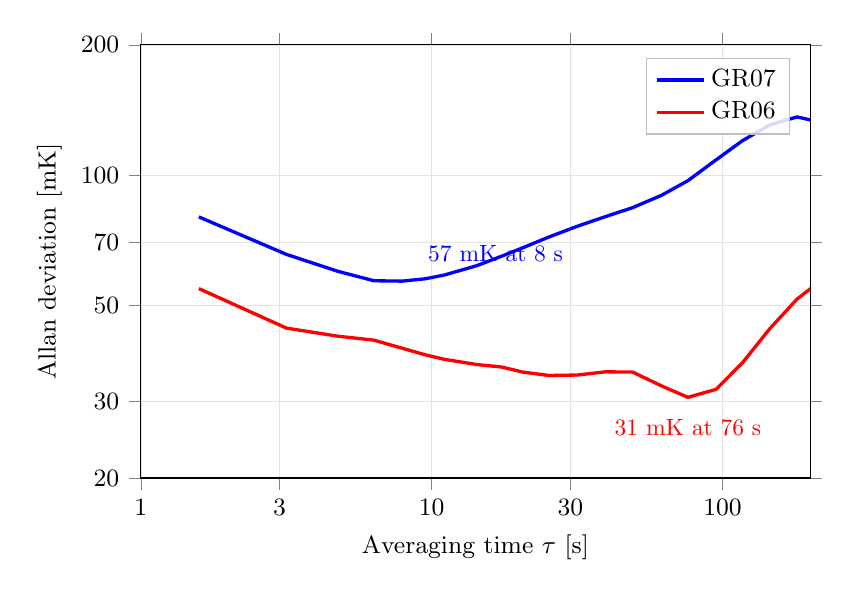
\begin{tikzpicture}[thick]

\begin{axis}[
  width=8.5cm,
  height=5.5cm,
  scale only axis,
  grid=both,
  grid style={gray!22, very thin},
  tick align=outside,
  tick label style={font=\small},
  label style={font=\small},
  title style={font=\small, yshift=-1mm},
  legend cell align=left,
  legend style={font=\small, draw=gray!50, fill=white, fill opacity=0.85, text opacity=1},
  xmode=log,
  ymode=log,
  xlabel={Averaging time $\tau$ [s]},
  ylabel={Allan deviation [mK]},
  xmin=1,
  xmax=200,
  ymin=20,
  ymax=200,
  legend pos=north east,
  log ticks with fixed point,
  ytick={20,30,50,70,100,200},
  xtick={1,3,10,30,100}
]
\addplot[blue, very thick, mark=none] coordinates {(1.5839,80.138) (3.1678,65.658) (4.7517,60.033) (6.3356,57.073) (7.9195,56.957) (9.5034,57.672) (11.087,58.871) (14.255,61.8) (17.423,65.054) (20.591,68.028) (25.342,72.047) (31.678,76.262) (39.597,80.269) (49.101,84.19) (61.772,89.928) (76.027,97.177) (95.034,108.54) (117.21,120.24) (145.72,130.77) (180.56,136.38) (224.91,131.84)};
\addlegendentry{GR07}
\addplot[red, very thick, mark=none] coordinates {(1.5839,54.745) (3.1678,44.371) (4.7517,42.506) (6.3356,41.612) (7.9195,39.877) (9.5034,38.5) (11.087,37.575) (14.255,36.571) (17.423,36.072) (20.591,35.117) (25.342,34.491) (31.678,34.575) (39.597,35.173) (49.101,35.118) (61.772,32.617) (76.027,30.707) (95.034,32.045) (117.21,36.919) (145.72,44.315) (180.56,51.8) (224.91,58.075)};
\addlegendentry{GR06}
\node[anchor=south west, blue, scale=0.85, align=left] at (axis cs:9.1074,60.375) {57 mK at 8 s};
\node[anchor=north, red, scale=0.85, align=left] at (axis cs:76.027,28.558) {31 mK at 76 s};
\end{axis}

\end{tikzpicture}
\end{document}
